\def\year{2020}\relax

\documentclass[letterpaper]{article} %DO NOT CHANGE THIS
\usepackage{aaai20}  %Required
\usepackage{times}  %Required
\usepackage{helvet}  %Required
\usepackage{courier}  %Required
\usepackage{url}  %Required
\usepackage{graphicx}  %Required
\frenchspacing  %Required
\setlength{\pdfpagewidth}{8.5in}  %Required
\setlength{\pdfpageheight}{11in}  %Required
\setcounter{secnumdepth}{0}  
\usepackage{subfigure}
\usepackage{enumerate}

\begin{document}
% The file aaai.sty is the style file for AAAI Press 
% proceedings, working notes, and technical reports.
%
\title{Replace This With Your Exciting CS 486/686 Project Title}
\author{Jane Smith\\
jane.smith@uwaterloo.ca\\
University of Waterloo\\
Waterloo, ON, Canada\\
}
\maketitle

%%%%%%%%%. Abstract %%%%%%%%%

{\bf For the proposal, please comment out any sections for the final report.}

\begin{abstract}
{\bf Complete the abstract for the final report.}

The abstract should be 1-2 paragraphs long. It should be at most 1/2 of the left column of the first page of the paper.

This is a short summary of your entire paper. You should include all the components of your project --- the motivation, the problem, the methodology, and the main results and take-away message. Do not attempt to include all your results. Instead, think of this as a highlight and an advertisement for your paper. If you only have 1 minute to describe your paper to someone, what would you say to grab their attention and make them remember your paper?

\end{abstract}

%%%%%%%%%. Introduction %%%%%%%%%

\section{Introduction} 

{\bf Complete this section for the proposal.}

The {\it Introduction} section ($\sim$1 page) consists of two parts. First, you will describe the problem you want to solve and the motivation for tackling the problem. Second, you will provide a summary of your project. 

Motivate your entire paper. Describe the problem that you are solving at a high level. Why is this an important problem to tackle? If there is a solution to this problem, what are some potential real-world impacts of this solution? Try to give a compelling motivating story. If possible, support your argument with evidence such as facts and statistics. 

Describe the research question you are trying to answer. The research question describes the specific question you want to answer/address in this project. The question usually involves a comparison. You may want to compare two different algorithms. If you are evaluating one main algorithm, you will want to compare the algorithm to a baseline method. You can use the baseline method to establish a minimum performance that your main algorithm must achieve. The baseline method serves as a sanity check that your main algorithm is performing at a reasonable level.

Your description of the research question should answer the following questions.
\begin{enumerate}
\item What problem are you going to solve? (e.g., build a ML model to classify whether a book review is positive or negative.)

\item What main algorithm(s) will you implement or modify to solve the problem? (e.g. transformer-based models: BERT and RoBerta)

\item What other baseline methods will you use for comparison to evaluate the performance of the main algorithm(s)? (e.g. variants of RNNs: LSTM)
\end{enumerate}
  
Here is an example of a research question: Will an AI agent based on [...] (the algorithm(s)) achieve higher/lower [...] (a quantifiable metric) compared to a model based on [...] (the selected baseline model)?
  
Here is an example of a research question: The research question our project will address is: Will an AI agent based on [...] (the algorithm(s)) achieve higher/lower [...] (a quantifiable metric) compared to a model based on [...] (the selected baseline model)?

Next, describe your methodologies. Briefly explain your main algorithms and baseline methods (1-2 sentences). Briefly explain how you adapt the algorithm to solve your problem.

Next, describe how you will evaluate the algorithms/models. What experiments will you carry out? What data-set will you use? What performance measure will you compute? 

\begin{enumerate}
  \item If the result is evaluated on a data-set:
    \begin{enumerate}
      \item What is the performance metric (e.g. accuracy/precision/recall/f1 score...)?
      \item Are you going to use an existing data-set or collect data by yourself? For an existing data-set, please cite the source. If you are going to collect the data by yourself, briefly explain how you are going to collect the data.
    \end{enumerate}
  \item If the result is evaluated in a simulated environment:
    \begin{enumerate}
      \item What are some features of the environment? Describe briefly and leave the details to D2. 
      \item Are you going to implement it or are you going to use an existing implementation?
      \end{enumerate}
    \item If the result is evaluated on user study:
        \begin{enumerate}
            \item What is the format of the user study? online questionnaire/user interview...
            \item Who will participate in the user study?  
            \item What is the most important question in this user study?
        \end{enumerate}
\end{enumerate}
 
{\bf Complete the following parts for the final report. }

{\bf Main Results}

Summarize your results. This part should be 1-2 paragraphs long.

{\bf Contributions}

Describe your contributions. This section should be around 1 paragraph long. 

Please list your 3-4 contributions in bullet points with an order of significance. You can make contributions to methodological research (e.g., the first paper to apply the algorithm xx to the problem of xx), or to the implementation (e.g., collected the data-set / implemented xx). It can be something big (e.g., our method beat the state-of-the-arts on multiple data-sets), or something small (e.g., we modified the code so that it can run on google cloud.). Some examples include:
\begin{itemize}
    \item We collected the data-set on ...
    \item We are the first to apply the algorithm xx on the domain xx
    \item We implemented the algorithm xx for xx 
    \item We compared the performance of algorithm xx and xx on the problem xx.
    \item We found a positive correlation between xx and xx.
    \item Our method achieves the best performance on the data-set xx
    \item Our implementation reduces the training time by xx.
    \item We modified the implementation of xx in order to ...
\end{itemize}

For each contribution, try to describe it at a high level in one sentence. Don't go into details. You don't have to be the first or the best at something on this planet to make contributions. However, if you really are, please be proud to say so and highlight!


%%%%%%%%%. Related Work %%%%%%%%%

\section{Related Work} 

{\bf Complete this section for the proposal.}

The {\em Related Work} section should be around 1 page long.

Summarize prior work for addressing the same problem or similar problems. 

You should aim to survey around 10-12 published papers. 

Whenever possible, synthesize the literature by describing multiple papers in aggregate, i.e., mentioning a common technique that multiple prior work used. 

Try to connect the prior work into a coherent story. Imagine that you are describing a story to someone about how researchers have used different techniques to solve the same or similar problems over time. 

Please use BibTeX to do citations. Here are some examples \cite{SS14,Block62,Novikoff62}.

%%%%%%%%%. Methodology %%%%%%%%%

\section{Methodology}

{\bf Complete this section for the proposal.}

The {\em Methodology} section should be around 2 pages long.

Describe the algorithms that you are planning to use to tackle your research question. If you are comparing multiple algorithms, describe each algorithm in detail. If you are evaluating one algorithm, make sure you describe the benchmark algorithm that you will use to evaluate the algorithm. 

Describe how each algorithm works in detail. Include their mathematical formulations, if necessary. Include pseudo-code, if necessary. If you had to change an existing algorithm for your problem, describe the changes in details. Assume that your reader only has a rudimentary knowledge of the algorithm. You should give enough details so that someone else can replicate your work given the description.

Explain why you selected these particular algorithms and how they are appropriate for solving the problem. 

\medskip
Describe the experiments you will conduct to answer your research question. 
\begin{itemize}
    \item Which algorithms will you compare? 
    \item What parameter values will you use? 
    \item If you are using cross-validation, how will you split up the data set into training, validation and test sets?
\end{itemize} 
Provide specific values for your choices. These values could change later. For now, you are making a plan about what values you will be trying. If you struggle with justifying your choices (e.g. a parameter value for a neural network), one valid reason is that a related work (provide a citation) used these parameter values and obtained good results. 

Describe how you will evaluate the performance of your algorithms. For example, are you going to look at the convergence time? Are you going to execute it on the problem and measure the total reward obtained? Are you going to look at the precision and recall? 

\medskip
If you are tackling a machine learning problem, you may need to evaluate your algorithm using a data set. You may use an existing data set or create a new data set yourself. 

If you use an existing data-set, make sure that you describe the following aspects.
\begin{itemize}
    \item Where did the data-set come from? (include the URL of the websites)
    \item How and why was the data set collected? 
    \item Why did you choose this data-set? Why is this data-set appropriate for your problem? What are its limitations?
    \item Size of the data-set (\# of data points, \# of features)
    \item What information does this data-set contain? Describe all the features and their types. Describe any other unique characteristics of the data-set.
    \item Data pre-processing (e.g. joining multiple data-sets, filtering out certain examples, scaling features). Explain why you are using these data preparation procedures.
\end{itemize}

If you are creating a new data set, make sure that you describe the following aspects.
\begin{itemize}
\item Why did you decide to create a new data-set instead of using an existing data-set? 
\item How will you collect the data?
\item What information will you collect?  
\item How many data points will collect?
\item Optional: any privacy and ethics concern?
\end{itemize}


%%%%%%%%%. Results %%%%%%%%%

\section{Results}

{\bf Complete this section for the final report.}

The {\it Results} section ($\sim$2 pages) describes the experiment results to help answer your research question.

Please describe the following parts in this section.
\begin{enumerate}[(a)]
    \item The design of your system (include UML diagrams if possible). Any technical challenges that you have encountered with your implementation and your data-sets and how you overcome those challenges. Your effort to optimize the performance of your implementation.
    \item The performance of your algorithms. Your effort to improve the performance of your algorithms. Detailed analyses of the hyper-parameters if possible. A qualitative analysis of how the performance changed for different values of the hyper-parameters. If possible, describe how your techniques compare to prior work. 
    \item The lessons you have learned by working on the implementation. The lessons could be technical or otherwise.
\end{enumerate}

If your project is implementation heavy (i.e., you implemented most of the algorithms by yourselves), your result section may focus more on (a) Talk about the design of your code, the technical challenges of the implementations and your efforts to optimize the performance of the code. You still need to present your model performance for (b). However, we are more lenient on your result.

If your project mostly uses codes from an existing library or repository, your part (b) should be more extensive. Describe your efforts to improve the model performance. More specifically, if you are doing a machine learning project, please include data exploration and detailed hyper-parameter analysis. Data exploration should include any interesting insights or challenges from the data set. Hyper-parameter analysis should include figures or tables to show how the model's performance changes with different values of each hyper-parameter. 

Prepare figures (e.g., Figure \ref{fig:results2}) and tables (e.g., Table \ref{tab:results1}) to describe your results clearly. Make sure to label your figures and tables and explain them in the text. If you are comparing the performance of algorithms, include statistical tests to assess whether the differences are statistically significant. 

\begin{table}[h!]
    \centering
    \normalsize{
    \begin{tabular}{ l c }
    \hline
         Techniques & F-1 Score\\
         \hline
          Baseline & 0.80 \\
          Another Baseline & 0.76\\
          My Awesome Algorithm & {\bf 0.95}\\
         \hline
    \end{tabular}}
    \caption{example of a table summarizing the results}
    \label{tab:results1}
\end{table} 

\begin{figure}[htbp!]
  \centering
  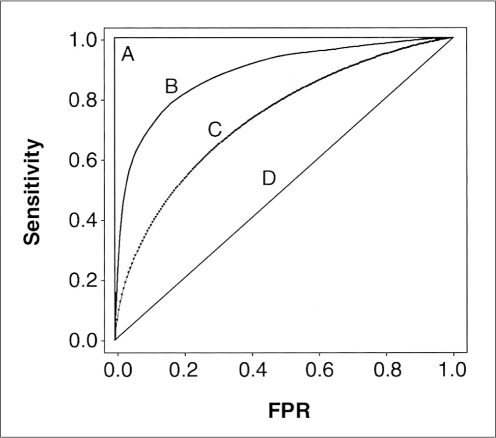
\includegraphics[width=0.9\linewidth]{figures/roc.png}
  \caption{ROC curve of my awesome algorithms}
  \label{fig:results2}
\end{figure}

%%%%%%%%%. Discussion %%%%%%%%%

\section{Discussion}

{\bf Complete this section for the final report.}

The {\em Discussion} section should be around 1 page long.

In this section, you will analyze the results. Here are 3 aspects you should cover (You are encouraged to use subsections to differentiate the contents):

Interpret your results: The meaning of the results might seem obvious to you, but it’s important to spell out their significance for the reader and show exactly how they answer your research questions. The form of your interpretations will depend on the type of research, but some typical approaches include:
\begin{itemize}
    \item Explain how results answered your research questions. 
    \item Discussing whether the results met your expectations or hypothesis (In line with the hypothesis…/ Contrary with the hypothesis...)
    \item Explaining unexpected results and evaluating their significance.
\end{itemize}

Discuss the implications: As well as giving your own interpretations, make sure to relate your results back to the scholarly work that you surveyed in D1. The discussion should show how your findings fit with existing knowledge, what new insights they contribute, and what consequences they have for theory or practice. 

\begin{itemize}
    \item Do your results agree with previous research? If so, what do they add to it? (These results build on existing evidence of…)
    \item Are your findings very different from other studies? If so, why might this be? (The results do not fit with previous work that…)
    \item Are there any practical implications? (Our project may help automate the process of ...)
\end{itemize}

Acknowledge the limitations: Even the best research has some limitations, and acknowledging these is important to demonstrate your credibility. Limitations are not about listing your errors, but about providing an accurate picture of what cannot be concluded from your study. Some examples can be:
\begin{itemize}
    \item Due to the limited computational resource we had, we were unable to test all possible hyper-parameters. Therefore, we acknowledge that our final setting may not be optimal.
    \item Our model can only be used to predict the popular vote for the US election. It is different from the electoral college in the actual election.
    \item Our sample size is too small or limited to a specific type of people, which will limit the generalizability of the results.
\end{itemize}

On the other hand, you should NOT cover the following.

\begin{itemize}
    \item Don’t introduce new results: you should only discuss the data that you have already reported in the result section.  
    \item Don’t make inflated claims – avoid over-interpretation and speculation that is not supported by your data.
    \item Don’t undermine your project – the discussion of limitations should aim to strengthen your credibility, not emphasize weaknesses or failures.
\end{itemize}

%%%%%%%%%. Conclusion %%%%%%%%%

\section{Conclusion}

{\bf Complete this section for the final report.}

The {\em Conclusion} section should be around 0.5 page long.

The conclusion is another mini-summary/recap of your paper. Write about the problem, motivation, and methodology briefly. Then summarize your results and the main takeaway messages. Finally, describe 2-4 future directions. See below for some examples of future directions.

\begin{itemize}
    \item "We would like to try these other hyper-parameters for these reasons"
    \item "It would be interesting to try a different model .... because ..."
    \item "The related problem .... is interesting because"
    \item "A different data processing method may be useful because ..."
\end{itemize}

%%%%%%%%% Bibliography %%%%%%%%%
\newpage
\bibliographystyle{aaai}
\bibliography{report}

\end{document}
